% Crucial Preamble
\documentclass[12pt,letterpaper]{article} \usepackage{amsmath} \usepackage{graphicx} \usepackage[margin=1in]{geometry} \usepackage{longtable}  \usepackage{amssymb}

% Extra Preamble
\usepackage{fancyhdr} \usepackage{enumitem} \usepackage{float} \usepackage{soul}
\usepackage{multicol} \usepackage[compact]{titlesec}


% frames with display breaks
\usepackage{mdframed}
\allowdisplaybreaks

% change spacing
\usepackage{setspace}
\setlength{\parskip}{0.4\baselineskip}

% Remove paragraph indentation
\setlength{\parindent}{0pt}

% Reduce space before and after section headings
%\titlespacing*{\section}{0pt}{0.1\baselineskip}{0.2\baselineskip}

% changes font
%\renewcommand{\familydefault}{\sfdefault}

% adds header and footer
\pagestyle{fancy}
\fancyhead{} \fancyhead[C]{ELG 2136 Cheat Sheet} \fancyhead[L]{ELG2136} \fancyhead[R]{Owen Daigle}
\fancyfoot{} \fancyfoot[C]{\thepage}


\begin{document}
	
	\begin{center}
		\Large\textbf{ELG 2136 Cheat Sheet} \\
		\vspace{0.5em}
	\end{center}	

	\section{Physics}
	Electric Conduction can happen due to 2 different mechanisms. 
	\begin{enumerate}[]	
		\item Forced Drift (When an Electric Field is applied)
		\item Natural Diffusion (Free charges tend to move to less densely charged areas)
	\end{enumerate}

	We define \textbf{$J$} as the current density which is just $\frac{\text{total current}}{\text {area}}$. J can be calculated for Drift, or Diffusion but we need a few more things defined. 
	
	We define $n_i$ as the density of electrons/holes, which depends on the boltzmann constant $k$, the temperature T, and the material specific bandgap energy $E_g$. 
	\begin{align*}
		n_i = 5.2\times 10^{15} T^{\frac{3}{2}} e^\frac{-E_g}{2kT}
	\end{align*}

	We define $q$ as the charge of a single electron/hole, $\mu_n, \mu_p$ as the mobility constants of the electrons (n) and holes (p), $D-n, D_p$ as the diffusion constants, $n$ and $p$ are the electron and hole concentrations, and $E$ is the electric field applied.
	\begin{align*}
		J_{drift} = q(\mu_n n+ \mu_p p) E \qquad J_{diffusion} = qD_n \frac{dn}{dx} - qD_p \frac{dp}{dx}
	\end{align*} 

	\subsection{Doping}
	While pure silicon is neutral, we can dope the silicon with boron (extra proton) or phosphorus (extra electron).
	
	We define $n_n, p_p$ as the number of free electrons and protons in a material at thermal equilibrium.
	
	If the material has majority positive (p-type), we say: $n_p, p_p, p_p\cdot n_p = n_i^2$
	
	If the material has majority negative (n-type), we say: $n_n, p_n, p_n\cdot n_p = n_i^2$
	
	We can put a p-type and n-type material adjacent, and that creates a \textbf{diode}.
	
	\section{Circuit Analysis with Diodes}
	We have three models for diodes. There is the ideal, constant voltage (ideal with voltage source), and constant voltage with resistance (ideal with voltage source and resistance). All of these model the real diode. 
	\begin{center}
		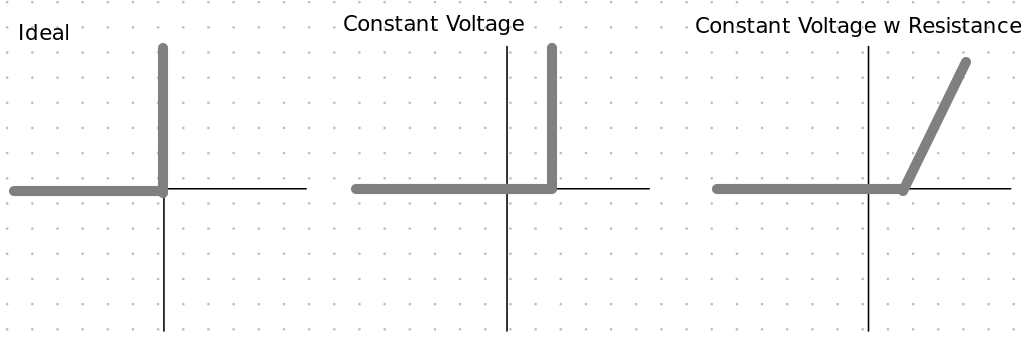
\includegraphics[width=0.8\linewidth]{diode-models}
	\end{center}

	An ideal diode can be either in the ON state (where current passes through in the correct direction) or the OFF state (where it acts as an open circuit). The other models just have this ideal diode with the voltage and resistance in series. 
	
	To determine the state of the diode, we need to assume a state (OFF or ON) and then check if it makes sense.
	\begin{itemize}[]
		\item If it is ON, then current MUST go from anode to cathode.
		\item If it is OFF, then voltage at cathode must be HIGHER than voltage at anode. 
	\end{itemize}

	If either of these criteria are wrong, then our assumption is on, and we need to try another one. 
	
	NOTE: There can only be \textbf{one } combination that works with a circuit. So if we have 2 diodes, and the first try it works, then it MUST be ONLY that combination.
	
	\begin{mdframed}[]
		\textbf{Ex. }
	\end{mdframed}
	
	\subsection{Plotting}
	For these problems, we have a circuit, and we have an input voltage (x axis) and another value such as output voltage, or output current, and we need to plot the output as a function of the inputs. 
	
	This is a lot of work since we have diodes, and when each diode changes, as will the relation between the input and the output. 
	
	This is the procedure: 
	\begin{enumerate}[noitemsep]
		\item Replace all diodes with their model (Ideal, Constant Voltage, CV with Resistance)
		\item Assume very low value for X (input) and find the state of each diode using this low value.
		\item Analyse the circuit to find Y (output) as a function of X (input)
		\item Find out which diode will switch its state \textbf{first }(let ON diode current=0, or OFF diode voltage=0)
		\item Replace the diode whose state changes first with its new state and \textit{return to step 3}. 
		\item STOP analysis once no more diodes will change state (diodes only change states at most 1 time).
	\end{enumerate}

	\begin{mdframed}[]
	\textbf{Ex. }
	\end{mdframed}
	
	\section{DC Power Supply}
	
	\subsection{Rectifier}
	The rectifyer will take an AC source, and make the output be positive.
	\begin{center}
		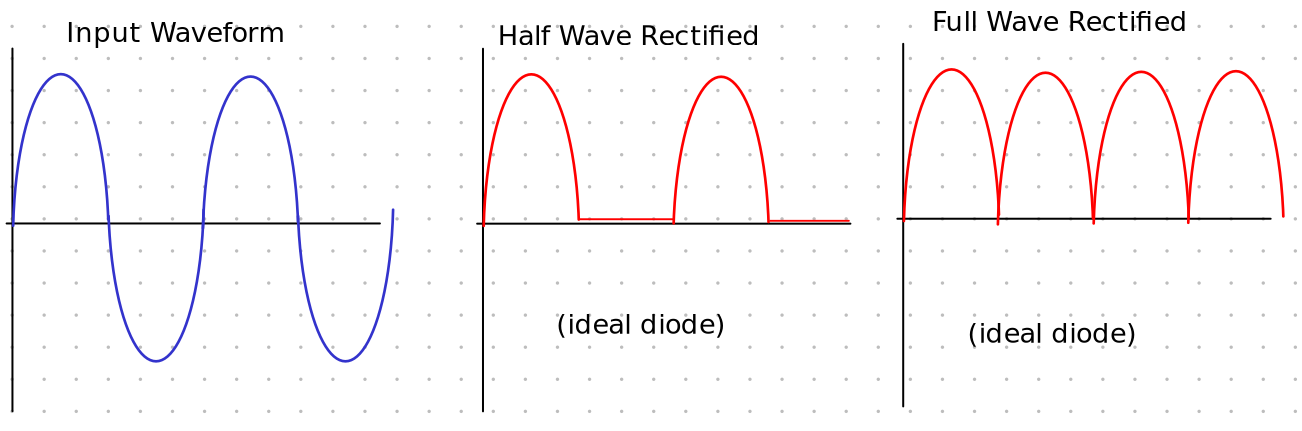
\includegraphics[width=0.9\linewidth]{rectifier}
	\end{center}
	
	
	A Half wave rectifier (1 diode) will just kill the negative part of the wave, while a Full wave rectifier (2 diodes) will keep the positive part, and invert the negative part. 
	
	A Bridge rectifyer is a special type of full wave rectifier that has 4 diodes instead of 2. 
	
	A useful statistic is the PIV (Peak Inverse Voltage) across a diode. To find this, we take a diode that we want to find the PIV across, then we find what would be the maximum negative voltage across this diode (note the diode will be OFF) when the source is at its inverse peak. 
	
	Typically we di a KVL through the circuit. Note that we find the voltage across the whole diode (including voltage and resistance if using that model).
	
	\begin{mdframed}[]
	\textbf{Ex. }
	\end{mdframed}
	
	\subsection{Filter}
	The Filter is just adding a capacitor in parallel with the load resistor. This will smooth out the big inflections, but there will still be a ripple. 
	\begin{center}
		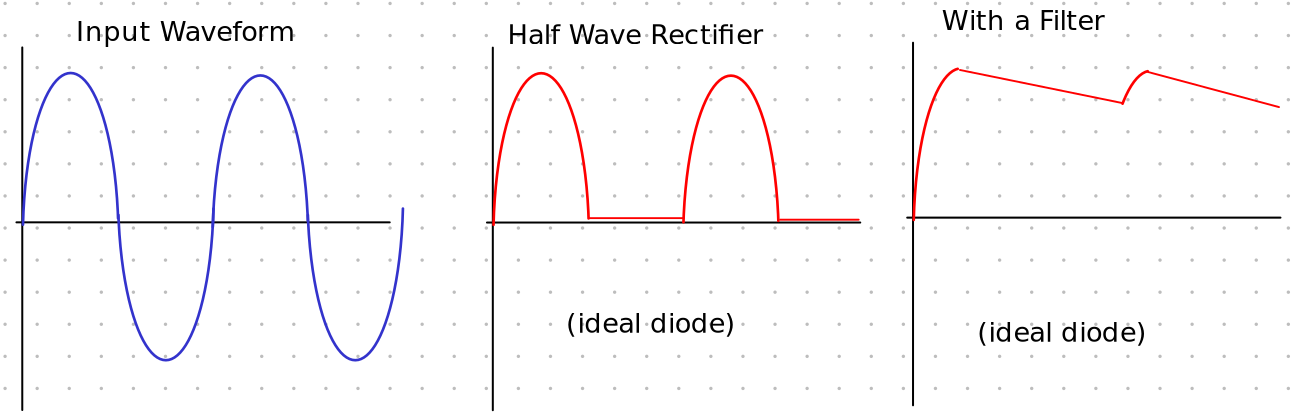
\includegraphics[width=0.9\linewidth]{filter}
	\end{center}

	We call $V_p$ the peak voltage of the wave, $V_r$ as the ripple voltage (if it fluctuates between 9 and 11 V, then $V_4=2V$), and $V_k$ as the minimum voltage.
	\begin{align*}
		V_p = V_k + V_r
	\end{align*}
	We can make some approxmiations (with ideal diodes) to see that:
	\begin{align*}
		V_r = \frac{V_p}{fRC} \text{ for a half wave rectifier or } V_r = \frac{V_p}{2fRC} \text{ for a full wave }\\
		\omega\Delta t = \sqrt{\frac{2V_r}{V_p}} \text{ for both types of rectifiers}\\
		\text{Current through diode average }i_{Davg} = I_L(1+\pi\sqrt{\frac{2V_p}{V_r}}) \text { for half wave or for full wave } \\ i_{Davg} = I_L (1+\pi\sqrt{\frac{V_p}{2V_r}}) \\
		\text{Current through diode MAX }i_{Dmax} = I_L(1+2\pi\sqrt{\frac{2V_p}{V_r}}) \text { for half wave or } i_{Dmax} = I_L (1+2\pi\sqrt{\frac{V_p}{2V_r}})\\
	\end{align*}

	If we are working with a different model, such as the constant voltage model, then we will need to modify the equations such as increasing the peak voltage by 0.7V. The one exception is the conduction angle formula $\omega \Delta t$ since that is not affected by te extra 0.7V.
	
	
	\subsection{Regulator}
	The regulator is a function that takes in a voltage source with unwanted ripples, and greatly reduces these ripples. It does this with a diode working in the breakdown region (zener diode).
	\begin{center}
		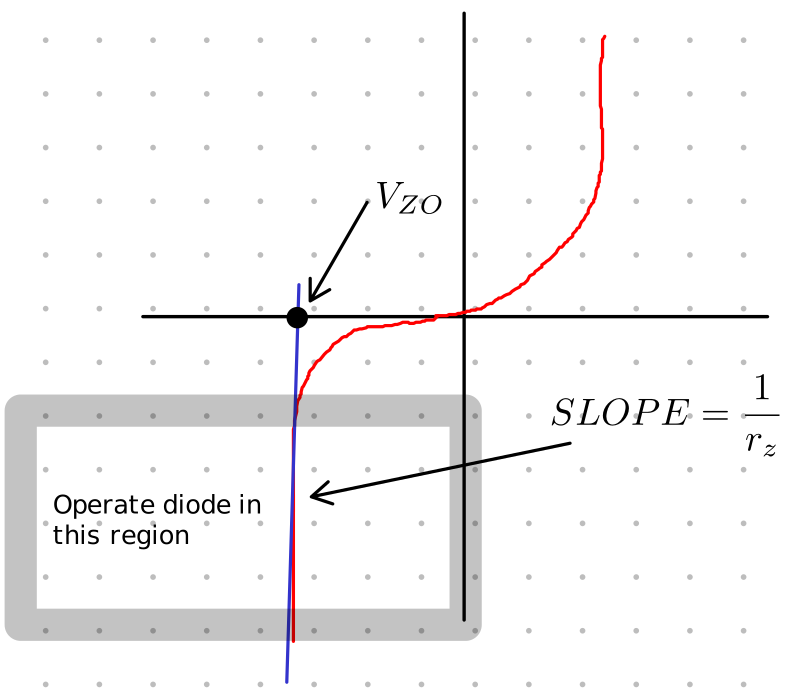
\includegraphics[width=0.4\linewidth]{regulator}
	\end{center}
	$r_z$ is the internal resistance of the diode. $V_{ZO}$ is the internal voltage source of the diode. 
	
	We need to ensure that the zener operates only in the breakdown region for no fluctuations in the output voltage. We do this by finding the minimum and maximum current allowed for the diode to stay in the breakdown region (straight line part).
	
	We want to maintain the output voltage to be as constant as possible, and this is measured using the line and load regulation. 
	\begin{align*}
		\text{Line Regulation}=\frac{\Delta V_O}{\Delta V_s} = \frac{r_z}{r_z+R} \qquad \text{Load Regulation}=\frac{\Delta V_O}{\Delta I_L} = -\frac{r_z\times R}{r_z+R} = -r_z // R
	\end{align*}

	\begin{mdframed}[]
	\textbf{Ex. }
	\end{mdframed}
	
	
	
	
	
\end{document}